\documentclass{bioinfo}
\copyrightyear{2015} \pubyear{2015}
\access{Advance Access Publication Date: Day Month Year}
\appnotes{Manuscript Category}
\usepackage{tikz}
\usepackage{graphicx}
\usepackage{amsmath}
\usepackage{float}
\usepackage{url}
\usepackage{multirow}

\begin{document}
\firstpage{1}

\subtitle{Genome analysis}

\title[popSTR]{popSTR: a population based microsatellite genotyper}
\author[Sample \textit{et~al}.]{Sn\ae d\'{i}s Kristmundsd\'{o}ttir\,$^{\text{\sfb 1,}*}$, Bjarni V. Halld\'{o}rsson\,$^{\text{\sfb 1,2}}$ and Birte Kehr\,$^{\text{\sfb 1}}$}
\address{$^{\text{\sf 1}}$deCODE genetics/Amgen, Reykjav\'{i}k, 101, Iceland and \\
$^{\text{\sf 2}}$Institute of Biomedical and Neural Engineering, Reykjav\'{i}k University, Reykjav\'{i}k, 101,
Icleand.}

\corresp{$^\ast$To whom correspondence should be addressed.}

\history{Received on XXXXX; revised on XXXXX; accepted on XXXXX}

\editor{Associate Editor: XXXXXXX}

\abstract{\textbf{Motivation:}Microsatellites, also known as short tandem repeats (STRs) are short DNA sequences containing repeated motifs ranging from 2-6 bases. 
There are about 700.000 microsatellites on the human reference genome covering almost 1\% of it \citep{eSTRgymrek} with the most common form being dinucleotide repeats.
The range of applications for microsatellite analysis is very wide and includes among other things medical genetics, forensics and genetic genealogy. However, microsatellite variations are rarely considered in whole-genome sequencing studies in large due to a lack of tools capable of analyzing them \citep{Duitama2014}.\\
\textbf{Results:} Here we present a microsatellite genotyper which is faster and more accurate than others previously presented. In order to accomplish this we utilize two things.
First, we reduce the amount of sequencing data necessary for creating microsatellite profiles when using previously aligned sequencing data. This is done by filtering the input to contain only reads aligned to known microsatellite locations and unaligned reads as these should be the ones useful for profiling.
Second, we use population information to train microsatellite and individual specific error profiles. 
Combining these two procedures we are able to give a practical implementation of microsatellite genotyping which is both faster and more accurate than previously presented solutions.\\
\textbf{Availability:} Code available on Github\\
\textbf{Contact:} \href{snaedis.kristmundsdottir@decode.is}\\
\textbf{Supplementary information:} Supplementary data are available at \textit{Bioinformatics}
online.}

\maketitle

\section{Introduction}
\label{s:intro}
Microsatellites have a mutation rate that is much higher than for other variations and its value has been estimated between $1 \cdot 10^{-4}$ and $1 \cdot 10^{-3}$ mutations per locus per generation \cite{sun2012direct}.
This high mutation rate is due to the repetitive structure of microsatellites which causes a secondary DNA conformation that makes replication slippage events more likely than in other locations of the genome \cite{Mirkin2007}. Replication slippage is an error which occurs when DNA molecules are copied. The error results in either an increase or decrease in the number of motif repeats. During replication the copy strand being created and the original template strand get shifted in their relative positions which causes a part of the template to either be copied twice or not copied at all, see Figure ~\ref{fig:RepSlipp}. As a result of this error the newly replicated polynucleotide has either an extra repeat unit or is missing a repeat unit \cite{Brown2002}.
The high mutation rate causes the alleles of a microsatellite to vary greatly between individuals \cite{sun2012direct} and no pair of individuals alive today have the same combination of alleles for all microsatellites \cite{Highnam2013}.
This makes it possible to create a unique genetic profile for every individual if enough microsatellites are profiled, with the exception of identical twins who share 100\% of their DNA \cite{NHGRI1999}.
There are a number of attributes which make the analysis of microsatellites using high throughput sequencing analysis pipelines hard. For a read to be useful for genotyping it must completely encompass the microsatellite. If a read only contains a portion of the microsatellite it can only give a lower bound on the number of repeats and thus only reads containing all of the microsatellite can be used for determining the number of repeats \cite{Gymrek2012}. Another challenge is how most popular read-to-reference aligners trade-off between the tolerance of insertions/deletions and running time.
Aligning a read to a reference genome becomes very hard if it contains a microsatellite, even if the microsatellite only has small number of added/deleted repeat motifs compared to the genome used as reference. This is due to the gaps that the extra/missing base pairs create in the alignment \cite{Li2010}. PCR amplification, a routine step in sample preparation for certain methods for whole genome sequencing, can create stutter noise. When this happens the DNA amplicons contain a false repeat length caused by successive slippage events during amplification. It results in reads declaring a false allele which damages the results of genotyping \cite{Ellegren2004}. The conclusion to be drawn from this is that despite its desirability, the analysis of microsatellites is challenging using the sequencing and analysis techniques available today.
\begin{figure}[ht]
\centering
 \includegraphics[width=0.5\linewidth]{figures/replicationSlippage.eps}
  \caption[Replication Slippage]{An extra repeat element added because of replication slippage \cite{Brown2002}.}
 \label{fig:RepSlipp}
\end{figure}


%\enlargethispage{12pt}

%\section{Approach} Is it necessary to include this section?

\begin{methods}
\section{Methods}

The popSTR process has 3 steps. During the first step we identify the reads useful for genotyping, compute their attributes and initialize genotypes. In the second step we compute an individual-specific slippage rate, quantifying the probability of a replication slippage event in this individual. In the third and last step we compute a marker specific slippage rate to quantify the probability of a replication slippage event at this marker, we train a logistic regression classifier for each marker and we perform genotyping.
\enlargethispage{6pt}
\subsection{Mathematical models}
\subsubsection{Slippage rate estimation}
The frequency of slippage errors that cause stutter noise varies between microsatellites. To account for this we estimate a specific slippage rate for each location. This gives an accurate estimation since it includes the characteristics of each microsatellite instead of using the same expression for all of them. We estimate the slippage rate at microsatellite $i$ by dividing the number reads at the microsatellite marked as error reads by the total number of reads aligned to the microsatellite.
The following expression is used to estimate $S^M_i$, the slippage rate at microsatellite $i$
\begin{equation}
    S^{M}_i = \frac{\sum n^e_i}{\sum n_i}
\label{eq:SmInit}
\end{equation}
where $n^e_i$ stands for the number of reads at microsatellite $i$ marked as error reads and $n_i$ stands for the total number of reads aligned to microsatellite $i$.
This expression however ignores the contribution of the individual to the slippage rate and considers only the microsatellite contribution.
To increase the accuracy of our slippage rate estimates, we update the expression of the estimate to contain the sum of slippage that is caused by the microsatellite location and the slippage that is caused by the individual.
A system of equations is used to estimate the slippage rate. Here, $S_{ij}$ represents the slippage rate for the pair of microsatellite $i$ and individual $j$, $S^{M}_i$ represents the slippage contributed by microsatellite $i$ and $S^{P}_j$ represents the slippage that individual $j$ contributes.
\begin{equation}
    S_{ij} = S^{M}_i+S^{P}_j 
\end{equation}
We denote the probability that a read aligned to microsatellite $i$, marked as an error read is actually reporting a true allele as $p^e_i$. The probability that a read aligned to microsatellite $i$, regardless of how it is marked, reports a true allele is represented by $p_i$. For reads grouped by individuals we let $p_{ij}$ denote the probability of reporting a true allele for a read aligned to microsatellite $i$ from individual $j$. To estimate the slippage rate at microsatellite $i$ we then use the following expression
\begin{equation}
S^{M}_i = \frac{\sum p^e_i}{\sum p_i} - 
\sum_j S^{P}_j \cdot \frac{\sum p_{ij}}{\sum p_i}
\label{eq:sMjEq}
\end{equation}
In the expression used for estimating the slippage of individual $j$ we let $p^e_j$ denote the probability that an error read from individual $j$ reports a true allele and $p_j$ denote the probability that a read from individual $j$ reports a true allele, regardless of how it is marked. So the expression becomes 
\begin{equation}
S^{P}_j = \frac{\sum p^e_j}{\sum p_j} - 
\sum_i S^{M}_i \cdot \frac{\sum p_{ij}}{p_j}
\label{eq:sPjEq}
\end{equation}
Although this estimate improves the previous expression it results in very high slippage rate estimates in some cases because all individuals contribute equally to the slippage at each position and vice versa without regard to their variance. If an individual or a microsatellite has a high variance they will then cause an overestimation of the slippage rate.
To decrease the weight of individuals and microsatellites with noisy reads in the slippage rate estimates we update the estimate again and weigh the contributions of each individual and microsatellite with the inverse of their variance. This gives microsatellites and individuals with low variance higher weights in the estimate and should thus make it more stable and reliable. 
The slippage rate at a microsatellite essentially represents the probability of getting an slippage error read at the given microsatellite and it is a binary distributed variable. We define the variance of a microsatellite as its slippage rate and use the definition of a variance for one trial on a binary distributed variable, given by
\begin{equation}
v = p(1-p)
\end{equation}
After this update, the expression for the slippage rate at microsatellite $i$ becomes 
\begin{equation}
S^{M}_i = \frac{\sum p^e_i}{\sum p_i} - 
\sum_j S^{P}_j \cdot 
\frac{ \frac{1}{S^{P}_j(1-S^{P}_j)} \cdot \frac{\sum p_{ij}}{\sum p_i}}{\sum_j \frac{1}{S^{P}_j(1-S^{P}_j)} \cdot \frac{\sum p_{ij}}{\sum p_i}}
\label{eq:sMiEq2}
\end{equation}
and similarly the slippage rate for individual $j$ becomes 
\begin{equation}
S^{P}_j = \frac{\sum p^e_j}{\sum p_j} - 
\sum_i S^{M}_i \cdot
\frac{ \frac{1}{S^{M}_i(1-S^{M}_i)} \cdot \frac{\sum p_{ij}}{\sum p_j}}
{\sum_i \frac{1}{S^{M}_i(1-S^{M}_i)} \cdot \frac{\sum p_{ij}}{\sum p_j}}
\label{eq:sPjEq2}
\end{equation}
Using these estimates we include the overall slippage rate of the individual or microsatellite being considered along with the contribution of each microsatellite to the individual and the contribution of each individual to the microsatellite. These contributions are however weighed with the inverse of their variance so noisy individuals or microsatellites will not skew the estimates.

\subsubsection{Modelling slippage and genotyping}
\label{subsubsec:modelSlipp}
To determine a genotype for individual $j$ at microsatellite $i$ we start by looking at all reads for the given individual aligned to the given microsatellite and determine the possible genotypes they offer. We then compute the likelihood of the reads given each genotype and pick the genotype that maximizes this likelihood. The expression used to compute this likelihood for a set of reads $R = \{r_1,\dots,r_n\}$ and a genotype $gt$ is 
\begin{equation}
P(\text{R|gt}) = \prod_s p(r_s|gt)
\end{equation}
Like the slippage rate estimates, the expression used to compute $p(r_s|gt)$ was updated several times. Our first version assumes a Poisson distribution of the stutter noise error events with $\lambda = S_{ij}$ and includes the probability of reporting a true allele given to every read by the logistic regression classifier of the microsatellite it is aligned to. We let $p(r^t_s)$ denote the probability that read $s$ reports a true allele and $x$ stand for number of slippage events. The number of slippage events is defined as the difference between the number of repeats reported by the read and the number of repeats in the genotype. This gives the following expression for a homozygous genotype $A$.
\begin{equation}
p(r_s|A) = p(r^t_s) \cdot pois(x;S_{ij})
\label{eq:likelihood}
\end{equation}
and for a heterozygous genotype $(A,B)$ we compute the number of slippage events relative to both alleles in the genotype.
\begin{multline}
p(r_s|A,B) = \\
p(r^t_s) \cdot 
(\frac{1}{2} \cdot pois(x(A);S_{ij})+ \frac{1}{2} \cdot pois(x(B);S_{ij}))
\end{multline}

The problem with this expression is that it becomes very small for non-slippage error reads. For these reads our model assumes that each of the other reported alleles is equally likely, so we set $n^i_{alleles}$ as the number of alleles present in the population for microsatellite $i$ and update the expression for $p(r_s|gt)$ in the following way

\begin{equation}
p(r_s|A) = p(r^t_s) \cdot pois(x;S_{ij}) + \frac{1-p(r^t_s)}{n^i_{alleles}}
\label{eq:likelihood2}
\end{equation}
and in the same way for a heterozygote genotype 
\begin{multline}
p(r_s|A,B) = p(r^t_s) \cdot (\frac{1}{2} \cdot pois(x(A);S_{ij})+ \\
\frac{1}{2} \cdot pois(x(B);S_{ij})) + \frac{1-p(r^t_s)}{n^i_{alleles}}
\end{multline}
Using this expression to determine the probability of a read given a genotype we assume that stutter noise is equally likely to result in reads with fewer repeat units and reads with extra repeat units. This is however not the case as stutter noise is more likely to delete repeat units and to account for this we add a parameter, $a$. The probability of deleting a repeat unit is set as $p_d$ and of adding a repeat unit as $p_a$ which means we set $a$ as $p_d$ if allele$_i < A$ and $p_a$ if allele$_i > A$ The expression derived from this thus becomes 
\begin{equation}
p(r_s|A) = p(r^t_s) \cdot pois(x;S_{ij}) \cdot a + \frac{1-p(r^t_s)}{n^i_{alleles}}
\label{eq:likelihood3}
\end{equation}
and in the same way for a heterozygote genotype but there we need $a_1$ and $a_2$ to compare allele$_i$ with both alleles of the genotype, $A$ and $B$
\begin{multline}
p(r_s|A,B) = p(r^t_s) \cdot \\
(\frac{1}{2} \cdot pois(x(A);S_{ij}) \cdot a_1+ \frac{1}{2} \cdot pois(x(B);S_{ij})\cdot a_2)\\
+ \frac{1-p(r^t_s)}{n^i_{alleles}}
\label{eq:likelihood3.5}
\end{multline}

Slippage events resulting in a non-unit addition or removal of the motif however should not be modelled in the same way as slippage events adding or removing a full copy of the motif. Because of this we model non-unit slippage events as following a geometrical distribution where $p = \frac{1}{\bar{x}+1}$ and $\bar{x}$ is the average step size modulo the length of the repeat motif \cite{Gymrek2012}.
To reflect this we update our heterozygous genotyping expression in the following way:
\begin{multline}
    p(r_s|A,B) = p(r^t_s) \cdot \\
    \biggl(\frac{1}{2} \cdot pois(floor(x_A);S_{ij}) \cdot geom(x_A-floor(x_A);p) \cdot a_1 \\ + \frac{1}{2} \cdot pois(floor(x_B);S_{ij})\cdot geom(x_A-floor(x_A);p) \cdot a_2 \biggr) \\
    + \frac{1-p(r^t_s)}{n^i_{alleles}}
    \label{eq:likelihood4}
\end{multline}
This final expression combines the power obtained both through the logistic regression classifier and the estimation of slippage rates at microsatellites and individuals. By adding the probability that a read is an error to the number it contributes to the likelihood we raise the tolerance for error reads. This makes it possible to call a homozygous genotype despite having perhaps a number of reads supporting another allele if these other reads get poor results from the logistic regression classifier.
\end{methods}
\section{Algorithm}
\subsection{Read selection}
    The read selection simultaneously scans through the sequencing data and the microsatellite location file and compares all reads to the current microsatellite coordinates. If a read intersecting a microsatellite is found it is stored along with its mate. When we reach reads with an alignment location greater than the current microsatellite coordinates we move on to the next microsatellite.
    \paragraph{\textbf{Pseudocode}} 
    We let $r_i^s$ and $r_i^e$ denote the start and end positions of the alignment for read number $i$, respectively. We set $m_j^s$ and $m_j^e$ as the start and end positions of microsatellite number $j$, respectively. For properties regarding the read we let $r_i^u$ be a logical value which is true if read $i$ is unaligned, $r_i^q$ be set to true if the read passes quality checks and $r_i^d$ be set to true if the read is an optical duplicate. Both the reads and microsatellites must then be sorted in the same way such that $\forall i,k$ if $i<k$ then $r_i$ comes before $r_k$ and $\forall j,l$ if $j<l$ then $m_j$ comes before $m_l$ in the sorting.
    Given sequencing data containing reads $r_1 \dots r_n$ and a microsatellite location file containing the genomic coordinates of microsatellites $m_1 \dots m_b$ we will start with $j=1$, consider each read from $1$ to $n$ separately and check for the following conditions
    \begin{enumerate}
        \item Is $r_i^q$ = FALSE? If yes, discard it and set $i = i+1$.
        \item Is $r_i^d$ = TRUE? If yes, discard it and set $i = i+1$.
        \item Is $r_i^u$ = TRUE? If yes, check the location of its mate and store both if the mate satisfies any of conditions 6-9, set $i = i+1$.
        \item Is $r_i^e$ \textless $m_j^s$? If yes, discard it and set $i = i+1$.
        \item Is $r_i^s$ \textgreater $m_j^e$? If yes, set $j=j+1$ and start from 4. again.
        \item Is $r_i^e \geq m_j^s$ and $r_i^e \leq m_j^e$? If yes, store $r_i$ and its mate and set $i = i+1$.
        \item Is $r_i^s \geq m_j^s$ and $r_i^s \leq m_j^e$? If yes, store $r_i$ and its mate and set $i = i+1$.
        \item Is $r_i^s \geq m_j^s$ and $r_i^e \leq m_j^e$? If yes, store $r_i$ and its mate and set $i = i+1$.
        \item Is $r_i^s \leq m_j^s$ and $r_i^e \geq m_j^e$? If yes, store $r_i$ and its mate and set $i = i+1$.
    \end{enumerate}
    
    \begin{figure}[H]
        \centering
        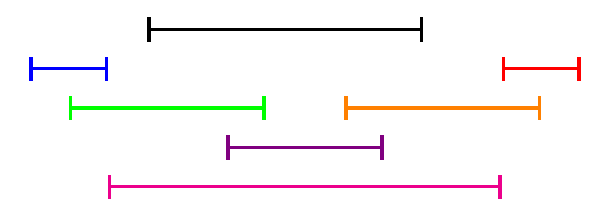
\begin{tikzpicture}
            \draw [|-|, black, very thick] (1.5,2) -- (5,2);
            \draw [|-|, blue, very thick] (0,1.5) -- (1,1.5);
            \draw [|-|, red, very thick] (6,1.5) -- (7,1.5);
            \draw [|-|, green, very thick] (0.5,1) -- (3,1);
            \draw [|-|, orange, very thick] (4,1) -- (6.5,1);
            \draw [|-|, violet, very thick] (2.5,0.5) -- (4.5,0.5);
            \draw [|-|, magenta, very thick] (1,0) -- (6,0);
        \end{tikzpicture}
        \caption[Method for selecting reads]{The black line at the top shows the microsatellite region. Condition 4 deals with the blue read, condition 5 with the red one, condition 6 with the green one, condition 7 with the orange one, condition 8 with the purple one and condition 9 with the pink one.}
    \end{figure}
    
    \noindent When a possibly useful read has been identified we check whether it contains the microsatellite it was aligned to. If it does, we align the flanking sequences of the repeat to the flanking sequences of the microsatellite, which we get from the reference genome and compute various attributes.
    After scanning through all reads we initialize genotypes based on frequencies.
\subsection{Logistic regression and genotyping}
    We train a logistic regression classifier for each microsatellite. The purpose is to account for errors not caused by stutter noise. We train the classifiers using only reads reporting true alleles and error reads not thought to result from stutter noise. Each read is assigned a probability of reporting a true allele by classifying it using the classifier trained for the microsatellite it covers. By including this probability in the slippage rate estimation expressions and in the expression used to determine the genotype and we attempt identify non-slippage error reads as well.
\section{Implementation}
PopSTR was written in C++ using the sequence analysis library SeqAn which allows for easy reading and manipulation of data stored in BAM-files \cite{Doering2008}.
\subsection{Read selection}
    We use the fact that the sequencing data has already been aligned and it is therefore possible to consider only reads aligned to known microsatellite locations along with unaligned reads. The unaligned reads are included since we don't know if they contain microsatellites or not. Sequences already aligned to non-microsatellite sequences are unlikely to be useful while sequences that are unaligned may in fact contain a microsatellite but have not been aligned because they are too different from the reference. We ran the Tandem Repeat Finder to determine the microsatellite locations \cite{TRF}.
    
    As mentioned before, when a useful read has been detected we align the flanking sequences of the repeat in the read to the microsatellite flanking sequences, which we get from the reference genome. The quality of this alignment is used as an indicator of how reliable the read is when performing genotyping. The purity of the repeat sequence in the read must also reach a minimum value for the read to be used and this minimum value is relative to the purity of the microsatellite sequence in the reference.
    
    To address the challenge presented by reads only able to give a lower bound on the number of repeats we allow for a user-specified maximum $m_l$. If the repeat occurs at either end of a read or spans the entire read and the base-pair length of the repeat is larger than $m_l$ we report the number of repeats as:
    \begin{equation}
        \frac{m_l}{lengt(repeatMotif)}
    \end{equation}
    These cases however require higher purity values from the the repeat and a minimum alignment score from the flanking sequences when they are available.(see exact numbers in Table ~\ref{table:numConditions}) 
    This gives the user the option to lump all alleles above a certain length into a "greater-than" allele.
    
    The following table summarizes the numerical values used as conditions in various cases during the read selection.
    \begin{center}
        \begin{table}[H]
            \caption{Minimum numeric values when identifying useful reads}
            \begin{tabular}{p{0.5\linewidth}|p{0.5\linewidth}}
                \hline
                \textbf{Name - Condition} & \textbf{Minimum value} \\ \hline
                Purity - standard case & 0.75*(ref. purity) \\ \hline
                Purity - no flanking & 0.85*(ref. purity) \\ \hline
                Purity - one sided flanking & 0.8*(ref. purity) \\ \hline
                Matching flank-bases fraction-one sided flanking & 0.7 \\ \hline
                Number of repeats - motiflength = 2 & 4 \\ \hline
                Number of repeats - motiflength = 3 & 3 \\ \hline
                Number of repeats - motiflength $\in {4,5,6}$ &  2\\ 
                \hline
            \end{tabular}
            \label{table:numConditions}
        \end{table}
    \end{center}
    
    We throw away low quality reads, i.e. the ones that fail platform or vendor quality checks and reads that are PCR or optical duplicates. This should increase the result quality since the reads being removed could possibly decrease the genotyping accuracy.
    When we have scanned all of the sequencing data and computed attributes for all useful reads at every microsatellite, we initialize genotypes based on frequencies and write both the attributes and the genotype initialization to an output file.
\subsection{Slippage computation - PN and marker specific}
    The slippage for individual $j$ is initialized by dividing the number of reads reporting an allele not in the initialized genotype by the total number of reads.
    \begin{equation}
            S^{P}_j = \frac{\sum n^e_j}{\sum n_j}
    \end{equation}
    When marker specific slippage rates have been computed and probabilities from logistic regression assigned to all reads, we update our estimate according to equation ~\ref{eq:sPjEq2}
    All probabilities in the marker slippage estimate expression given in equation ~\ref{eq:sMiEq2} are initialized as 0.95 but in later iterations they are computed for each read by plugging its attributes into the logistic regression classifier of the microsatellite they were aligned to.
\subsection{Logistic regression classifier and genotyping}
    The logistic regression attributes used are various but all have in common their ability to indicate the quality of a read in one way or the other. These are summarized in Table ~\ref{table:attributes}. 

    \begin{table*}[ht]
        \caption{The attributes used as control variables in the Logistic regression classification.}
        \begin{tabular}{p{0.5\linewidth}|p{0.5\linewidth}}
            \hline
            \textbf{Attribute} & \textbf{Definition} \\ \hline
            Quality score & Map quality score of the aligned read. \\ \hline
            Purity & \# of repeats in the microsatellite sequence/ 
            \# of expected repeats in the microsatellite sequence \\ \hline
            Number over 20 in & The number of bases in the read with a PHRED quality over 20 in the microsatellite sequence. \\ \hline
            Number over 20 after & The number of bases in the read with a PHRED quality over 20 coming after the microsatellite sequence. \\ \hline
            Edit distance of mate & Edit distance to the reference, including ambiguous bases but excluding clipping. \\ \hline
            Alignment score before & Alignment score of sequence before the microsatellite to the reference. \\ \hline
            Alignment score after & Alignment score of sequence after the microsatellite to the reference. \\ \hline
            Was unaligned & Boolean value indicating if the read was unaligned. \\ \hline
            Location shift & Measures alignment shifting during the realignment of flanking sequences. \\ \hline
            Sequence length & Total length of the read-sequence. \\
            \hline
        \end{tabular}
        \label{table:attributes}
    \end{table*}
    
    Having assigned a probability to all reads and estimated the slippage rates at all microsatellites and for all individuals we now have what we need to determine the genotypes. To do this for individual $j$ at microsatellite $i$ we follow the process described in Section ~\ref{subsubsec:modelSlipp}. Probabilities of deletion or addition in Equation ~\ref{eq:likelihood4} were set as $p_d = 0.85$ and $p_a = 0.15$. 
\subsection{Data set}
 While training we iterate between steps II and III until convergence has been reached. In 2015, popSTR was run on around 8000 individuals for around 700.000 microsatellites. We chose a training set of 8303 microsatellites based on their good results from imputation into the Icelandic population. Training was performed using 703 individuals with high quality sequencing data.
 Using results from the training to directly estimate slippage rates for new individuals on these 8303 microsatellites allows us to skip the training process in later genotyping. 
 Comparison with lobSTR was done by choosing 10 random individuals from the 15.220 sequenced individuals available at the time. We chose 146 markers where inhouse capillary electrophoresis benchmark genotypes were available and compared our and lobSTR genotypes to those.
 To further investigate the quality of our genotypes we matched our microsatellites coordinates to output coordinates and indel alleles from the GATK genotype caller and compared the imputation results into the Icelandic populations for markers where matching was possible. 
 
\section{Results}
\subsection{Training}
During the training 5 iterations were performed until convergence was reached. Figures ~\ref{fig:pnSlipp} and ~\ref{fig:markerSlipp} show the distribution of slippage rate values for the training set.
\begin{figure}[H]
\centering
 \includegraphics[width=\linewidth]{figures/pnSlippageHist.png}
  \caption[Histogram of pn-slippage]{Histogram of slippage rates for the 703 individuals in the training set.}
 \label{fig:pnSlipp}
\end{figure}

\begin{figure}[H]
\centering
 \includegraphics[width=\linewidth]{figures/markerSlippageHist.png}
  \caption[Histogram of marker-slippage]{Histogram of slippage rates for the 8303 microsatellites in the training set.}
 \label{fig:markerSlipp}
\end{figure}

\subsection{Running popSTR on 15.220 individuals}
A total of 380.261 microsatellites were imputed into the Icelandic population.
First, we performed step I and identified useful reads and computed their attributes for all PNs at all markers. Next, we directly estimated individual slippage rates using only reads aligned to the 8303 microsatellites from the training set. We used the logistic regression classifiers from the training to assign probabilities to the reads and plugged the probabilities into equation ~\ref{eq:sPjEq2} along with the marker slippage rates from training. 
As a sanity check of the individual slippage rates we checked if they correlate significantly with age. The slippage rate was expected to increase with age due to somatic mutations that accumulate throughout a persons life. Due to a sequencing method batch effect observed in the data we considered only individuals sequenced using HiSeqX machines. Despite this we observed a batch effect as a result of moving from methods using PCR amplification to PCR-free methods. We therefore included a boolean for this property in the age correlation test. The results from that were very clear that slippage rate increases with age (p-value=8.21e-13)
Last we genotyped all individuals using Equation ~\ref{eq:likelihood4}.

\subsection{Comparison to lobSTR}
We compared the popSTR genotypes and the lobSTR genotypes to inhouse benchmark data obtained through capillary electrophoresis. The comparison was done on a set of 10 individuals chosen at random and 146 microsatellites chosen due to the availability of data. 
Comparison was performed both considering all genotypes as well as considering only genotypes where 10 or more reads were available. Table ~\ref{table:lobSTRcomp} summarizes the results. 
\begin{table}[H]
    \caption{Accuracy comparison of lobSTR and popSTR with and without coverage filtering.}
    \begin{tabular}{ c | c | c | c | c |}
         & \multicolumn{2}{c}{No coverage filter} & \multicolumn{2}{c}{coverage $ \geq 10$} \\
         \hline
         & \# genotypes & accuracy & \# genotypes & accuracy \\
         \hline
        popSTR & 1138 & 92.5\% & 969 & 95.1\% \\
        \hline
        lobSTR & 1135 & 86.8\% & 647 & 91.2\% \\
        \hline
    \end{tabular}
    \label{table:lobSTRcomp}
\end{table}
\subsection{Comparison to GATK}
Compare imputation info of my genotypes from the big run to GATK calls for microsatellites matched by Brynja's program.
Histogram like in Brynja's report on where my info is higher and where lobSTR info is higher

\section{Discussion}

Here I will discuss problems, improvements and results. Such as not identifying fewer than x repeats (depending on motif length) and trying to find the optimal value for $m_l$. Mention that association will be run on these results ? 









%%%%%%%%%%%%%%%%%%%%%%%%%%%%%%%%%%%%%%%%%%%%%%%%%%%%%%%%%%%%%%%%%%%%%%%%%%%%%%%%%%%%%
%
%     please remove the " % " symbol from \centerline{\includegraphics{fig01.eps}}
%     as it may ignore the figures.
%
%%%%%%%%%%%%%%%%%%%%%%%%%%%%%%%%%%%%%%%%%%%%%%%%%%%%%%%%%%%%%%%%%%%%%%%%%%%%%%%%%%%%%%






\section{Conclusion}
Here we have shown that when creating a microsatellite profile for an individual using previously aligned data it is possible to significantly decrease the running time by considering only reads that are either aligned to a known microsatellite location or not aligned at all. This type of filtering dismisses a large portion of the data immediately without significantly effecting the microsatellite profile. To do this we used the alignment locations of reads along with attributes indicating undesirable qualities.


\section*{Acknowledgements}
deCODE, Amgen ??? 

%\bibliographystyle{natbib}
%\bibliographystyle{achemnat}
%\bibliographystyle{plainnat}
%\bibliographystyle{abbrv}
%\bibliographystyle{bioinformatics}
%
\bibliographystyle{plain}
\bibliography{document}
\end{document}
